\documentclass[conference]{IEEEtran}
\usepackage{cite}
\usepackage{amsmath,amssymb}
\usepackage{graphicx}
\usepackage{booktabs}
\usepackage{url}
\graphicspath{{../figures/v4/}{../figures/phase2/}}
\begin{document}
\title{Route-Informed Reordering Tolerance and Its Loss-Recovery Costs in a LEO TCP Model}
\author{\IEEEauthorblockN{Team 5}
\IEEEauthorblockA{Independent study draft for team review\\
CS30401 Introduction to Computer Networks, Fall 2026}}
\maketitle

\begin{abstract}
Forwarding changes in low Earth orbit (LEO) networks can let later TCP
segments overtake earlier ones. We investigate the supplied ns-3.48
CUBIC/SACK/PRR implementation and establish one unnecessary recovery using
transmission identities, receiver application acceptance, ACK/SACK
feedback, and drop traces. A temporarily raised packet-count loss threshold
removes the episode: first-event goodput improves by 1.4432\%, but
whole-run improvement is only 0.02256\%. The same protection delays a
20-MSS actual-loss transfer from 0.251510 to 1.150124 seconds. An upfront
exemption for known transfers of at most 21 nominal MSS restores their
baseline recovery while retaining the tested large-flow protection.
It still fails above the cutoff and does not eliminate last-segment
timeouts. A separate, loss-free 80-MSS delay-step control completes 29.53\%
earlier under protection. Across 23 initial and 52 additional declared
cases, we identify benefit and failure conditions rather than claim a
general LEO or modern Linux TCP improvement. Deployment additionally
requires timely route information and application transfer-size knowledge.
\end{abstract}
\begin{IEEEkeywords}
LEO networks, CUBIC, SACK, packet reordering, loss detection
\end{IEEEkeywords}

\section{Introduction}
LEO satellite motion changes feasible links and forwarding paths.
Even when connectivity remains available, a shorter new path can deliver
later packets before packets already using the old path. Hypatia
demonstrates the resulting unnecessary TCP window reduction in a packet-level
LEO simulation~\cite{hypatia}. This makes the loss-detection response to
forwarding changes a useful question distinct from interruption recovery.

Our question is: \emph{when does route-related reordering produce
unnecessary recovery in the course CUBIC/SACK/PRR stack, and what benefit
and genuine-loss cost follow from selective reordering tolerance?}
Related subquestions examine finite transfer size, activation timing,
queue capacity, and link rate. CUBIC is a standardized contemporary
congestion controller~\cite{cubic}; however, the inspected course stack
uses packet-count loss inference and lacks RACK-TLP. Our conclusions
concern this implementation, not current Linux TCP.

The contribution has three parts. First, we connect a concrete forwarding
transition to receiver-accepted originals that are subsequently
retransmitted. Second, we implement sender-side, scheduled threshold
protection and compare event-local gains with full-run costs. Third,
we expose feedback starvation in finite transfers and evaluate a
conservative known-size exemption, including its failing boundary.
The refinement preserves baseline detection for exempt flows rather
than inventing a new loss-recovery algorithm.

Reordering tolerance already has substantial prior art. TCP-NCR delays
recovery, adapts its threshold to connection state, and uses Extended
Limited Transmit to obtain feedback~\cite{ncr}. Early Retransmit addresses
small flights that cannot supply three duplicate ACKs~\cite{early}.
RACK-TLP instead uses transmission time and probes to handle reordering
and limited feedback~\cite{rack}. Our fixed scheduled threshold is
neither a complete NCR implementation nor an implementation of RACK.
The distinctive evaluation is its route-informed activation and
measured benefit/cost envelope in the supplied environment.

\section{Problem Statement}
\subsection{A verified unnecessary recovery}
We first reproduce the supplied Seoul--London scenario with CUBIC,
10-Mbit/s links and 100-packet device queues. Around the 26.2-second
forwarding update, the path changes from 12 to 10 hops; the geometric
two-direction propagation RTT decreases from 97.698 to 91.064 ms.
The RTT sum selects a candidate event, but receiver sequence evidence,
rather than geometry alone, establishes overtaking.

Figure~\ref{fig:causal} shows the causal episode. Original transmission
21,859, starting at TCP sequence 29,734,861, is accepted at
26.283909347 seconds with same-time receiver application delivery.
At 26.328788841 seconds, ACK 29,734,861 carries a SACK block
$[29{,}739{,}001,29{,}743{,}141)$, three MSS above the hole.
The inspected SACK presumed-loss rule reaches its default threshold of
three, marks the segment lost, and initiates recovery and retransmission.
This episode is not explained simply as three consecutive duplicate ACKs.
The cumulative ACK covering the segment, 29,736,241, reaches the sender
at 26.329936038 seconds: only 1.147197 ms after recovery starts.
The receiver had already accepted the original.

We join each transmission with a flow identifier, transmission identifier,
and transmit timestamp. No matching physical or queue drop is observed
for that original under the connected drop hooks. This is positive
acceptance evidence plus observed drop coverage; a wire arrival or
cwnd decrease alone would be insufficient. The event contains five
out-of-order payload arrivals and three retransmissions. Larger loss
thresholds remove those retransmissions while preserving delivery.

\begin{figure*}[t]
\centering
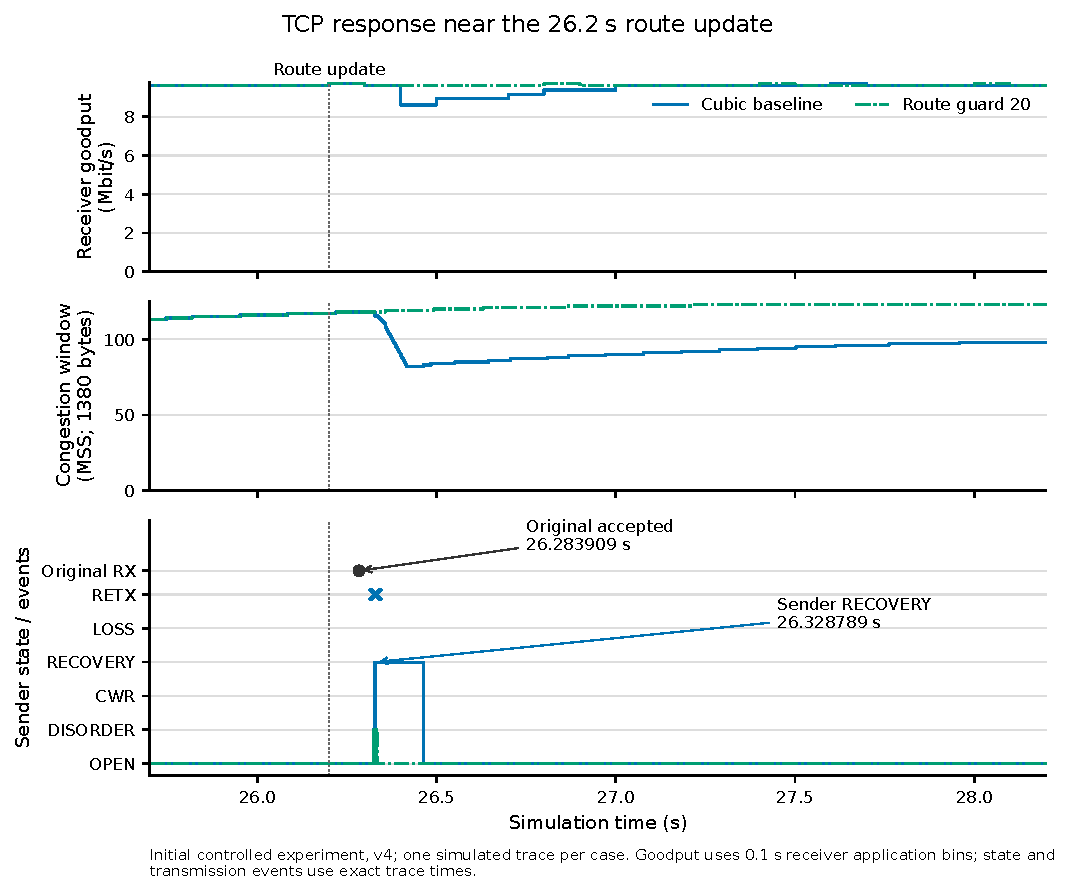
\includegraphics[width=\textwidth]{route_event_causal.pdf}
\caption{The original 26.2-second LEO event. Packet identities,
receiver delivery, ACK/SACK evidence and sender state establish
unnecessary recovery; geometric RTT and cwnd alone do not establish it.
All panels come from the same declared baseline/control cases.}
\label{fig:causal}
\end{figure*}

\subsection{Controls and the real-loss risk}
A routing-timing control holds the 26.1-second forwarding snapshot
through updates 26.2--26.8 and resumes current forwarding at 26.9.
Satellite motion and geometric propagation continue. Neither transition
reproduces the original recovery. This supports dependence on update
timing and the packets in flight, but does not isolate propagation delay
from every changed link or queue history.

Raising a packet-count threshold also postpones genuine-loss detection.
For a finite 20-MSS transfer with its first segment dropped once, a
threshold of 20 cannot obtain the same feedback as the default threshold
of three. The protected transfer completes at 1.150124001 seconds,
versus 0.251509920 seconds for baseline, about 4.57 times later.
Both deliver the same 27,600 bytes within the four-second run; average
goodput therefore hides the penalty. This is the feedback-starvation
tradeoff anticipated by NCR~\cite{ncr}, measured in our prototype.

\section{Proposed Idea(s)}
\subsection{Selective threshold activation}
The sender retains CUBIC's window-growth equation and changes the
packet-count threshold used in duplicate-ACK processing and SACK
presumed-loss marking. Baseline uses $K=3$. The initial selective policy
uses $K=20$ during requested intervals 26.1--26.5 and 74.9--75.3 seconds,
then returns to three. A continuous high-threshold baseline distinguishes
selective activation from simply increasing tolerance everywhere.

Activation does not erase existing SACK loss marks. It must precede the
relevant loss decision. Restoration runs after ACK processing and is
permitted in \texttt{CA\_OPEN} or \texttt{CA\_LOSS}; other states defer it.
The requested end is consequently not a hard bound on high-threshold
exposure. In the 20-MSS counterexample, the requested end is 0.5 seconds
but restoration occurs at 1.100009281 seconds after timeout. Updating
the threshold alone does not process a new ACK, reevaluate all pending
losses, or generate a retransmission when no feedback arrives.

\subsection{Upfront known-size exemption}
The refinement computes $N=\lceil B/M\rceil$ before connection
establishment, where $B>0$ is the application's known total byte count
and $M$ is its configured segment size. For cutoff $C=21$,
\begin{equation}
K_{\mathrm{effective}}(t)=
\begin{cases}
3, & B>0\ \text{and}\ N\le C,\\
K_{\mathrm{scheduled}}(t), & \text{otherwise}.
\end{cases}
\end{equation}
Open-ended transfers are not classified as small. The cutoff is an
exploratory conservative choice near $K=20$; the inclusive 21-MSS and
exclusive 22-MSS controls test its boundary. It is not a derived optimum.
Nominal MSS equivalents are not measured on-wire packet counts.

This policy does not inspect remaining flight, count future ACK
opportunities, or adapt on detecting a tail. It deliberately leaves
known small transfers on baseline loss detection and gives up their
possible reordering-protection benefit. Generic threshold-set trace
entries, including $3\rightarrow3$ on exempt flows, are not evidence of
an effective high-threshold interval.

\subsection{Information and deployment assumptions}
The prototype receives absolute protection times through configured
flow parameters. These are oracle schedules informed by the supplied
forwarding state; the sender does not predict routes itself. A prospective
operator could notify affected terminals or senders using planned
forwarding updates, their expected times, uncertainty and expiry.
That requires access to routing policy, affected-flow mapping, timely
delivery and compatible sender integration. Public satellite orbits
alone do not determine the actual forwarding policy.

Notification latency, clock error, cancellations, missing notices and
unscheduled rerouting remain deployment concerns. Wider protection can
cover uncertainty while increasing genuine-loss exposure. We test
shifted protection intervals, not a notice-delivery protocol. The
size exemption additionally requires application total-size knowledge,
available here as \texttt{MaxBytes}, which ordinary TCP streams may not
announce. No receiver wire-format change is needed in the prototype.
Timers and altered loss detection are sender costs; forecasting and
notification are operator costs. Message overhead and kernel integration
have not been measured. Research packet tracing is not proposed
production overhead.

\section{Experiment Setup}
\subsection{Environment and parameter bases}
We use the official \texttt{2026f-v1} Docker image, pinned by digest,
and its ns-3.48/Hypatia source; the source commit, image digest,
versioned patches and exact commands are recorded in the bundle.
The LEO state is the supplied Starlink shell 1 Seoul--London example
with 100-ms forwarding updates. We retain 1,380-byte segments,
initial cwnd of ten segments, and 32-MiB buffers. No random radio loss,
handover interruption or varying link capacity is added.

\begin{table}[t]
\caption{Important controlled parameter choices}
\label{tab:params}
\centering
\begin{tabular}{p{0.98in}p{2.17in}}
\toprule
Setting & Values and basis\\
\midrule
LEO rates/queues &
10 Mbit/s with 100 packets; 100 Mbit/s with 1,000.
Both give a payload-only per-device queue-time proxy of 110.4 ms.
50 packets tests a smaller queue.\\
Thresholds &
3 baseline; 8, 20, 32 at 10 Mbit/s; 64 in higher-rate
controls. Diagnostic sensitivity choices, not optima.\\
LEO duration &
200 s for supplied state; 85 s at 100 Mbit/s includes
both selected updates. A 100-GB transfer sustains load.\\
Protection &
400-ms LEO intervals: 100-ms lead and 300-ms follow-up.
Chosen from observed events, not a universal rule.\\
Finite controls &
100 Mbit/s, 2,000-packet queues, initial ssthresh 900 MSS,
approximately the 100-ms payload BDP (906 MSS).\\
Finite timing &
4-s observation; one-way 50 ms, optionally 45 ms after
0.201 s. $K=20$ over 0--0.5 s; cutoff 21.\\
\bottomrule
\end{tabular}
\end{table}

The rates and queues are controlled operating conditions, not deployed
Starlink measurements. Headers, ACKs and multiple hops prevent treating
the table's queue proxy as an end-to-end delay bound. The initial bulk
microbenchmark runs for 20 seconds and changes one-way delay from
50 to 45 ms at 10 seconds, or injects one loss on stable delay.
Its protection interval is 9.99--10.3 seconds with $K=64$.
Finite controls instead use transfer sizes 3, 4, 8, 20, 21, 22 and
80 nominal MSS. Selected middle and last losses test feedback position.
An exact sequence filter drops one specified original data segment once;
no intentional loss is installed in delay-step or stable no-loss controls.
The 0.201-second step was selected during pilot exploration to expose a
mixed packet phase around the channel change, not as a natural workload
arrival time. The 50-to-45-ms change gives a 10-ms propagation RTT decrease
near the LEO event's scale; the matched stable control separates geometry
from the TCP response. These are diagnostic choices rather than a fitted
satellite-delay model.

\subsection{Metrics, coverage and reproducibility}
Application goodput in Mbit/s is $8D/(10^6T)$, where $D$ is unique
delivered receiver application bytes and $T$ is the measurement interval
in seconds: the full run or the fixed 2.5-second event window.
Finite-flow completion time is final
unique application delivery minus application start at zero, including
connection establishment; it is recorded only after all requested bytes
arrive. Sender ACK progress and wire payload are separate measurements.
Event windows are fixed at 25.7--28.2 and 74.5--77.0 seconds, independent
of any shifted notification. Smoothed RTT is time-weighted between trace
changes and is not an isolated queue-delay measurement.

Transmission tags join sender, receiver and drop observations; repeated
drop-hook rows are deduplicated by transmission identity. Device, queue,
IP and traffic-control hooks are connected and root queue-disc absence
is checked. Receiver acceptance requires positive application or expected
sequence evidence. We do not claim every receiver rejection path is
audited. The large queues in finite controls avoid an automatic AQM
confound; drop traces still decide whether loss occurred.

There are 23 initial case IDs and 52 phase-two IDs: 31 finite actual-loss,
six finite no-loss, six finite delay-step, three bulk LEO and six nonzero
window offsets. Phase-two regressions overlap earlier conditions.
These 75 declared runs are deterministic configurations, not 75 unique
conditions or independent seed samples; no confidence intervals are
inferred. On an empty official source volume, applying and building
the canonical version-6 patch and replaying all 75 cases succeeds.
SHA-256 comparison matches all 600 raw/legacy input trace files and
75 full analysis files byte for byte. This verifies those deterministic
outputs; it is not an image-byte comparison or statistical replication.
The fresh simulation replay takes 377.093 seconds with at most three
concurrent runs; this excludes build, analysis, hashing and rendering.
The README maps manifests to commands and figures, pins plotting
dependencies, and distinguishes simulation, analysis and build runtime.
Raw traces and generated network state are excluded from the submission
bundle.

\section{Evaluation}
\subsection{LEO benefit is local and conditional}
With $K=20$ protection, first-event goodput rises from 9.485568 to
9.622464 Mbit/s, a 1.4432\% improvement. Its three retransmissions and one
recovery entry disappear. Over all 200 seconds, goodput changes from
9.5443560 to 9.5465088 Mbit/s, only 0.02256\%.
Continuous $K=20$ reaches 9.5469504 Mbit/s, slightly above selective
protection; selective protection is not the throughput winner.
The known-size refinement gives the same bulk result because the
100-GB transfer exceeds its cutoff.

Thresholds 8, 20 and 32 produce identical tested 10-Mbit/s results.
At 100 Mbit/s, threshold 64 improves whole-run goodput only 0.0064\%.
With 50-packet queues, first-event delivery improves by about 7.6\%,
but whole-run goodput decreases about 0.366\%. Mean SRTT is 148.13 ms
for the main baseline, 151.19 ms with selective protection and
154.95 ms with continuous protection. These are different congestion
trajectories, not proof of a fixed queue-delay increment caused by $K$.

The second event also limits the claim. Over 74.5--77.0 seconds, baseline
goodput is 9.626880 Mbit/s versus protected 9.618048 Mbit/s, and the
protected trajectory contains 12 retransmissions and two recovery
entries. Earlier behavior can alter later congestion and packet phase.
Protection does not improve both event windows or eliminate all recovery.

\subsection{Real loss and the exemption boundary}
\begin{figure}[t]
\centering
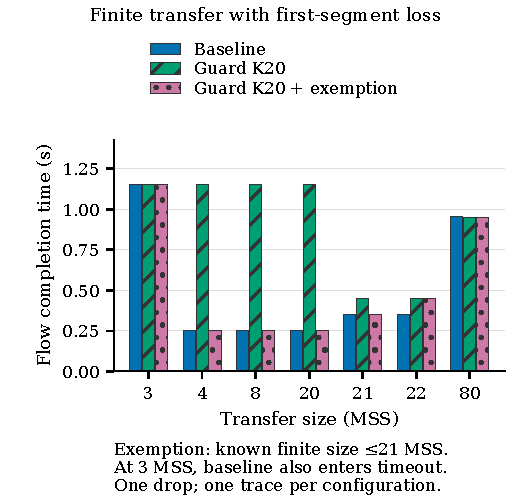
\includegraphics[width=\columnwidth]{finite_size_first_loss.pdf}
\caption{First-segment loss: completion time for baseline,
unqualified $K=20$ protection and the known-size exemption.
The exemption includes 21 MSS; the 22-MSS penalty remains.
The separate 20-MSS $K=8$ control is discussed in the text.}
\label{fig:size}
\end{figure}

All 31 finite actual-loss cases deliver their full requested bytes,
observe one intentional receive drop, and retransmit once.
Figure~\ref{fig:size} shows why those equal counts do not establish equal
application performance. At 20 MSS, the exemption restores baseline
0.251509920-second first-loss completion from protected 1.150124001.
For middle loss, it restores 0.350711200 seconds from 1.251165120.
The repair follows from bypassing the larger threshold, not faster
detection at $K=20$.

First-loss timing is also restored for the tested four- and eight-MSS
transfers. At exactly 21 MSS, baseline and exemption take 0.350482400
seconds versus protected 0.450716800. Immediately above the cutoff,
22 MSS takes 0.450716800 seconds under both protected policies,
versus baseline 0.350597120. Reducing $K$ to eight at 20 MSS avoids
the long timeout but still takes 0.350482400 seconds, 98.97248 ms
longer than baseline. Neither a smaller fixed threshold nor cutoff 21
solves finite-flight loss recovery generally.

With three MSS, all policies enter the timeout path and take
1.150124001 seconds: the baseline already lacks enough following
feedback~\cite{early}. Last-segment loss likewise takes
1.351284160 seconds at 20 MSS and 1.552210560 at 80 MSS under all
policies. Exemption cannot generate feedback after the last segment.
In a stable bulk-flow actual-loss control, $K=64$ postpones first
retransmission and validated gap repair by 6.99792 ms even though
whole-run goodput is unchanged. Actual protection extends to
10.4237584 seconds beyond its requested 10.3-second end.
That bulk control also observes 144 background traffic-control drops
besides its one injected physical drop. The timing comparison concerns
the matched injected target, not a globally loss-free bulk trajectory.

\subsection{A loss-free finite reordering control}
\begin{figure}[t]
\centering
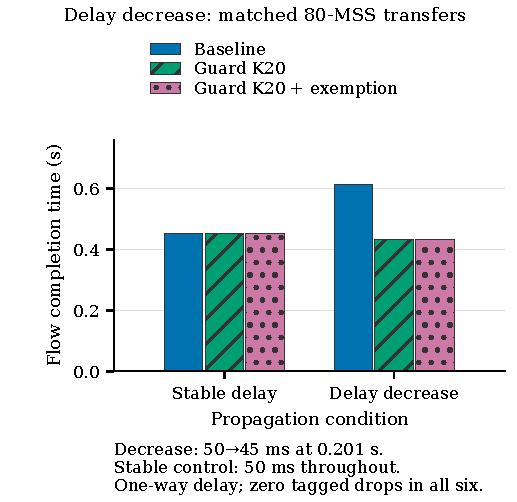
\includegraphics[width=\columnwidth]{finite_delay_step.pdf}
\caption{Finite completion on the same changed channel, with
matched stable-delay controls. The 80-MSS gain is a synthetic
delay-step result; it is not a whole-run LEO throughput gain.}
\label{fig:step}
\end{figure}

Figure~\ref{fig:step} evaluates a controlled 50-to-45-ms one-way
delay change at 0.201 seconds. At 20 MSS, all policies complete at
0.251050400 seconds without recovery. At 80 MSS, baseline completes
at 0.611527200 seconds with eight retransmissions and one recovery
entry; both protected variants complete at 0.430944960 seconds
with none, 29.53\% earlier on the \emph{same changed channel}.
The 80-MSS exemption does not activate. Matched stable-delay,
no-loss controls complete at 0.452206240 seconds under every policy,
without recovery. The shorter propagation alone therefore does not
explain the baseline's slower completion.

All eight retransmitted original ranges are accepted at
0.250247360--0.251050400 seconds before retransmission at
0.291399520--0.291973120. Higher sequence 24,841 arrives while the
receiver expects 13,801. Recovery at 0.291399520 coincides with the
third eligible repeated ACK and three SACKed segments above the hole;
unlike the main LEO episode, the duplicate-ACK and SACK branches are
not separately isolated. Covering ACK 15,181 arrives 3.8528 ms later.
No network drop is observed under the connected hooks. TCP timestamps
precede device service, so a packet affected by the channel change
need not have its TCP transmit timestamp after 0.201 seconds.
This control establishes an avoidable response in a deterministic
synthetic channel; it is not a measured LEO workload.

\subsection{Timing sensitivity and remaining limits}
\begin{figure}[t]
\centering
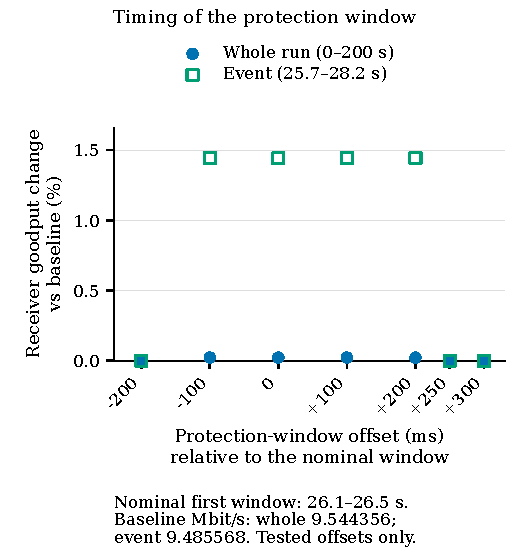
\includegraphics[width=\columnwidth]{protection_window_offset.pdf}
\caption{Both endpoints of both requested windows are shifted.
First-event delivery is evaluated at the fixed true event window.
The tested offsets demonstrate timing dependence rather than a
continuous or universal notification-accuracy bound.}
\label{fig:offset}
\end{figure}

Figure~\ref{fig:offset} shifts both LEO windows by the same offset,
retaining their 400-ms duration. Offsets $-100$, 0, $+100$ and $+200$ ms
retain the tested first-event benefit. At $-200$ ms, protection ends
before critical feedback; at $+250$ and $+300$ ms it begins after the
loss decision. These cases reproduce the baseline trajectory.
The discrete points do not prove every intermediate offset succeeds.
They do not model message transport, prediction errors or clock drift.

The study uses one supplied ground-station pair and predominantly one
flow. Multi-flow fairness, other paths, loss bursts and stochastic notice
errors remain untested. Very small reordered flights may benefit from
protection that our exemption relinquishes; the benign 20-MSS step
does not prove otherwise. An adaptive residual-flight policy, explicit
loss reevaluation or probe, and an implemented RACK-TLP comparison
would each require additional adverse controls. We do not present
initial Vegas/BBR throughput probes as validated alternative mechanisms.

\section{Conclusion}
In the supplied CUBIC/SACK/PRR stack, a forwarding transition triggers
recovery after original acceptance. Selective protection removes the
episode with 1.4432\% local but 0.02256\% whole-run gains.
Its 4.57-fold genuine-loss penalty motivates known-size exemption,
restoring tested small-flow baseline timing while retaining larger-flow
protection. The 21/22-MSS boundary, last-loss timeouts, adverse queues
and timing tests expose its limits. This reproducible tradeoff study
depends on operator information and transfer-size knowledge; it does
not establish a general improvement to deployed TCP.

\begin{thebibliography}{1}
\bibitem{hypatia}
S. Kassing, D. Bhattacherjee, A. B. Aguas, J. E. Saethre, and A. Singla,
\emph{Exploring the Internet from space with Hypatia}, in
\emph{Proc. ACM Internet Measurement Conference}, 2020, pp. 214--229.
\bibitem{cubic}
L. Xu, S. Ha, I. Rhee, V. Goel, and L. Eggert,
\emph{CUBIC for Fast and Long-Distance Networks}, RFC 9438, Aug. 2023.
\bibitem{ncr}
S. Bhandarkar, A. L. N. Reddy, M. Allman, and E. Blanton,
\emph{Improving the Robustness of TCP to Non-Congestion Events},
RFC 4653, Aug. 2006.
\bibitem{early}
M. Allman, K. Avrachenkov, U. Ayesta, J. Blanton, and P. Hurtig,
\emph{Early Retransmit for TCP and Stream Control Transmission Protocol
(SCTP)}, RFC 5827, Apr. 2010.
\bibitem{rack}
Y. Cheng, N. Cardwell, N. Dukkipati, and P. Jha,
\emph{The RACK-TLP Loss Detection Algorithm for TCP},
RFC 8985, Feb. 2021.
\end{thebibliography}
\end{document}
